Các ứng dụng web giống như những tảng băng trôi. Có một phần của ứng dụng mà người dùng nhìn thấy, tuy nhiên thì phần lớn nhất của ứng dụng vẫn là cái không nhìn thấy được - Backend. Nhiều công nghệ lập trình phía máy chủ đã ra đời và mỗi thứ đều có ưu điểm riêng. Mục tiêu của các công nghệ đó không chỉ giúp cho server chạy nhanh hơn mà còn đem lại trải nghiệm tốt hơn cho lập trình viên, giúp lập trình viên quản lý mã nguồn dễ hơn, debug dễ hơn, dễ tích hợp thêm tính năng mới hơn.
\subsubsection{Spring}
Spring là framework phát triển ứng dụng phổ biến nhất dành cho Java Enterprise. Spring có kích thướng nhẹ, phiên bản cơ bản của Spring framework có kích thước khoảng 2MB. Với Spring Framework các nhà phát triển có thể tạo ra các mã có hiệu suất cao, dễ kiểm thử và có thể sử dụng lại được.\par
Các tính năng core của Spring Framework có thể được sử dụng trong việc phát triển bất kỳ ứng dụng Java nào. Bên cạnh đó, phần mở rộng được sử dụng để xây dựng các ứng dụng web trên nền tảng Java EE. Mục tiêu của Spring Framework là làm cho việc phát triển ứng dụng J2EE dễ dàng hơn và thúc đẩy việc lập trình tốt hơn bằng mô hình POJO-based.
\begin{figure}[h!]
    \begin{center}
        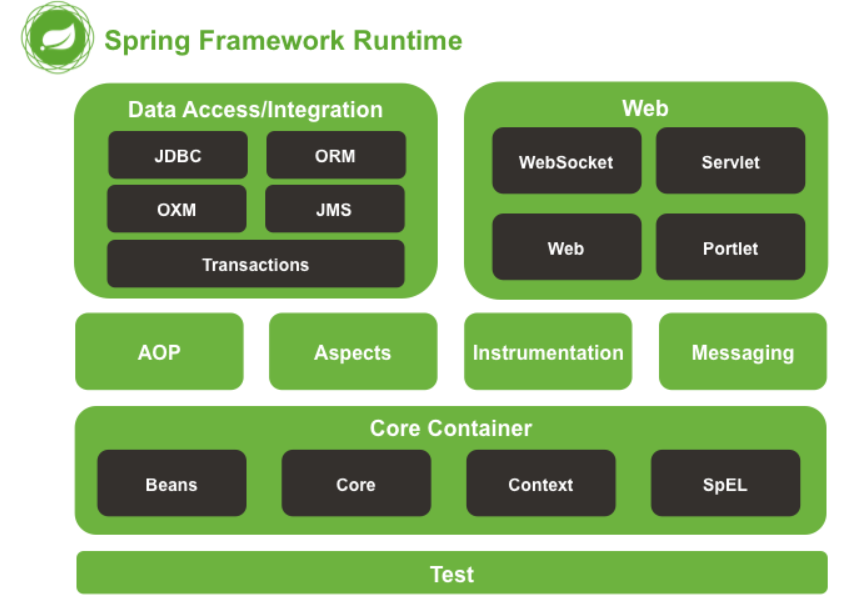
\includegraphics[width=10.8cm]{Image/Technical/spring_framework.png}
        \caption{Spring Framework}
        \label{spring}
    \end{center}
\end{figure}
\\
Ưu điểm của việc sử dụng Spring Framework:
\begin{itemize}
    \item Spring cho phép các nhà phát triển tạo các ứng dụng cấp Enterprise sử dụng các POJO. 
    \item Spring được tổ chức theo kiểu mô đun, dễ quản lí và phát triển.
    \item Dễ dàng để kiểm thử một chương trình được viết bằng Spring.
    \item Web framework của Spring là một Web MVC framework có thiết kế tốt, nó là một thay thế tuyệt vời cho Struts và các công nghệ kém phổ biến khác.
    \item IoC Container của Spring có trọng lượng nhẹ.
    \item Spring cung cấp một giao diện quản lý transaction nhất quán có thể mở rộng đến một local transaction.
\end{itemize}
Nhược điểm:
\begin{itemize}
    \item Không có một hệ sinh thái thư viện mạnh mẽ như các framework khác.
    \item Khó tiếp cận đối với người mới học lập trình web.
\end{itemize}

\subsubsection{Hibernate Framework}
Cơ sở dữ liệu quan hệ hướng đối tượng (Object-relational Database - ORD) là một hệ thống quản lý cơ sở dữ liệu (DBMS) bao gồm cả cơ sở dữ liệu quan hệ (RDBMS) và cơ sở dữ liệu hướng đối tượng (OODBMS). Cơ sở dữ liệu quan hệ đối tượng hoạt động như một giao diện giữa cơ sở dữ liệu quan hệ và hướng đối tượng vì nó chứa các khía cạnh và đặc điểm từ cả hai mô hình.\par

Cơ sở dữ liệu quan hệ hướng đối tượng (ORD) phục vụ hai mục đích chính:
\begin{itemize}
    \item Kết nối sự phân chia giữa cơ sở dữ liệu quan hệ và các kỹ thuật mô hình hướng đối tượng thường được sử dụng trong các ngôn ngữ lập trình như C\#, Java và C ++.
    \item Thu hẹp khoảng cách giữa các kỹ thuật mô hình hóa dữ liệu khái niệm cho cơ sở dữ liệu quan hệ và hướng đối tượng như sơ đồ entry-relationship (ERD) và ánh xạ quan hệ đối tượng (ORM).
\end{itemize}

Cơ sở dữ liệu hướng đối tượng (Object Oriented Database - OOD) được tổ chức xung quanh các đối tượng hơn là quan hệ, dữ liệu hơn là logic. Do đó, OOD là một hệ quản trị cơ sở dữ liệu trong đó thông tin được biểu diễn dưới dạng các đối tượng như được sử dụng trong lập trình hướng đối tượng (object).\par

Thông thường, khi OODBMS được tích hợp với một ngôn ngữ lập trình hướng đối tượng, sẽ nhất quán hơn nhiều giữa cơ sở dữ liệu và ngôn ngữ lập trình vì cả hai đều sử dụng cùng một mô hình biểu diễn dữ liệu. Khi so sánh với cơ sở dữ liệu quan hệ, cơ sở dữ liệu hướng đối tượng lưu trữ dữ liệu phức tạp, mối quan hệ giữa các dữ liệu trực tiếp mà không cần ánh xạ tới các hàng và cột như trong khi cơ sở dữ liệu quan hệ.\par

Sự khác nhau của Cơ sở dữ liệu hướng đối tượng (Object Oriented Database) và Cơ sở dữ liệu hướng quan hệ (Object Relational Database):\\

\begin{table}[h]
    \centering
    \begin{tabular}{|m{3cm}|m{5cm}|m{5cm}|}
    \hline 
        \textbf{Cơ sở so sánh} & \textbf{Object Oriented Database} & \textbf{Object Relational Database}\\ \hline
        Kết nối giữa hai quan hệ 
        & Các mối quan hệ được thể hiện bằng các tham chiếu thông qua mã định danh đối tượng (id).
        & Các kết nối giữa hai quan hệ được biểu diễn bằng các thuộc tính khóa ngoại trong một quan hệ tham chiếu đến khóa chính của một quan hệ khác.\\ \hline
        Cấu trúc lưu trữ dữ liệu 
        & Sử dụng các kỹ thuật lập chỉ mục để định vị các trang đĩa lưu trữ đối tượng. Do đó, chúng có thể cung cấp khả năng lưu trữ liên tục cho các đối tượng có cấu trúc phức tạp. 
        & Không chỉ định bất kỳ cấu trúc lưu trữ dữ liệu nào, mỗi quan hệ cơ sở được triển khai dưới dạng tệp riêng biệt và do đó, chúng không thể cung cấp khả năng lưu trữ liên tục cho các đối tượng có cấu trúc phức tạp.\\ \hline
        Số lượng dữ liệu 
        & Xử lý dữ liệu lớn hơn và phức tạp hơn.
        & Xử lý dữ liệu tương đối đơn giản hơn.\\ \hline
        Các ràng buộc 
        & Các ràng buộc được hỗ trợ bởi khác nhau với các hệ thống khác nhau. 
        & Nó có các khóa, tính toàn vẹn của thực thể và tính toàn vẹn của tham chiếu.\\ \hline
        Ngôn ngữ thao tác dữ liệu 
        & Thường được kết hợp với một ngôn ngữ lập trình như Java, C\#,... 
        & Có các ngôn ngữ thao tác dữ liệu như SQL, QUEL và QBE dựa trên quan hệ.\\ \hline
        Kiểu dữ liệu 
        & Có thể xử lý các loại dữ liệu khác nhau.
        & Có thể xử lý một kiểu dữ liệu duy nhất.\\ \hline
        Lưu trữ dữ liệu 
        & Dữ liệu được lưu trữ dưới dạng các đối tượng.
        & Dữ liệu được lưu trữ dưới dạng bảng, chứa các hàng và cột.\\
    \hline 
    \end{tabular}
    \caption{Object Oriented Database và Object Relational Database.}
    \label{OOD and ORD}
\end{table}

ORM (Object Relational Mapping) giúp đơn giản hoá việc tạo ra dữ liệu, thao tác dữ liệu và truy cập dữ liệu. Đó là một kỹ thuật lập trình để ánh xạ đối tượng vào dữ liệu được lưu trữ trong cơ sở dữ liệu. Hibernate framework là một giải pháp ORM mã nguồn mở, gọn nhẹ. Hibernate giúp đơn giản hoá sự phát triển của ứng dụng java để tương tác với cơ sở dữ liệu.\\
 \begin{figure}[h!]
    \begin{center}
        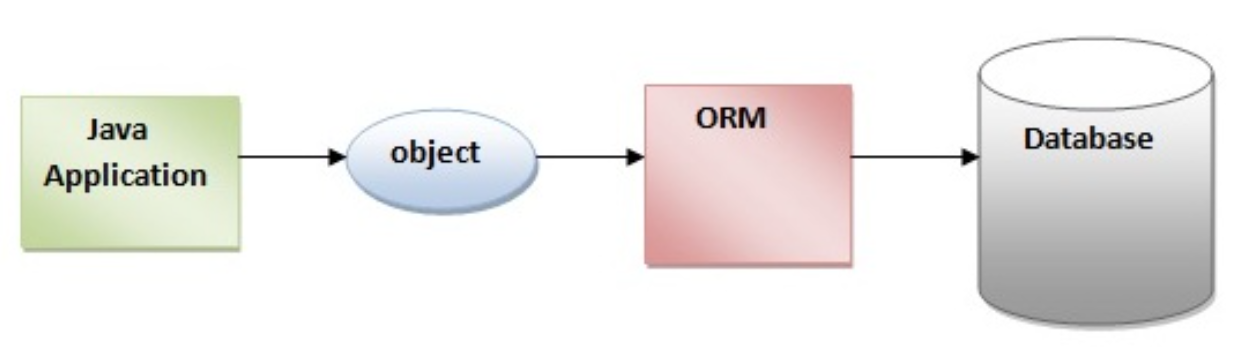
\includegraphics[width=15cm]{Image/Technical/hibernate_module.png}
        \caption{Mô hình Hibernate}
        \label{spring}
    \end{center}
\end{figure}

Hibernate Framework có các ưu điểm như dưới đây:
\begin{itemize}
    \item Mã nguồn mở và nhẹ.
    \item Hiệu suất nhanh.
    \item Truy vấn cơ sở dữ liệu độc lập.
    \item Tạo bảng tự động.
    \item Đơn giản lệnh join phức tạp.
    \item Cung cấp thống kê truy vấn và trạng thái cơ sở dữ liệu.
\end{itemize}
Bên cạnh đó Hibernate Framework ccũng có các nhược điểm:
\begin{itemize}
    \item Không hỗ trợ các câu truy vấn phức tạp.
    \item Một số trường hợp vẫn phải dùng native SQL do Hibernate không thể cover hết tất cả các cú pháp của các hệ quản trị cơ sử dữ liệu.
    \item Bị hạn chế sự can thiệp vào câu lệnh SQL do nó được tự động sinh ra.
\end{itemize}

\subsubsection{JPA Query Language}
JPA (Java Persistence API) thực hiện nhiệm vụ ánh xạ giữa các đối tượng Java với cơ sở dữ liệu quan hệ, sử dụng ORM (Object Relational Mapping).\par

JPA hoạt động như một cầu nối giữa các quan hệ trong database với các đối tượng Java, có thể persist một đối tượng Java vào trong cơ sở dữ liệu hoặc lấy dữ liệu từ cơ sở dữ liệu và ánh xạ ra các đối tượng Java. Các công cụ của JPA cho phép chúng ta thực hiện điều đó một cách đơn giản và nhanh chóng.\par

Spring Boot JPA là một phần trong hệ sinh thái Spring Data, nó tạo ra một layer ở giữa tầng service và database, giúp chúng ta thao tác với database một cách dễ dàng hơn, tự động config và giảm thiểu code thừa thãi.\par

Khi sử dụng JPA, chúng ta có thế:
\begin{itemize}
    \item Viết ít code hơn, nhưng vẫn có được performance tốt.
    \item Độc lập về database, không phải làm việc trực tiếp với các quan hệ.
\end{itemize}

\subsubsection{RESTful API}
API (Application Programming Interface) là tập các quy tắc và cơ chế để một thành phần ứng dụng có thể tương tác với một thafnh phần ứng dụng khác. API có thể trả về dữ liệu ở những kiểu dữ liệu phổ biến như JSON hay XML cho ứng dụng.\par

REST (REpresentational State Transfer) là một kiểu kiến trúc chuyển đổi cấu trúc dữ liệu cho API. REST sử dụng phương thức HTTP đơn giản cho giao tiếp giữa các thành phần ứng dụng. Thay vì sử dụng một URL cho việc xử lý một số thông tin người dùng, REST bao gồm các thao tác như GET, POST, DELETE,... đến một URL để xử lý dữ liệu.\par

RESTful API là một tiêu chuẩn dùng trong việc thiết kế các API cho các ứng dụng. RESTful API được sử dụng phổ biến rộng rãi ngày nay cho web, mobile… vì tính tiện lợi và hiệu uqar của nó.\par

\begin{figure}[h!]
    \begin{center}
        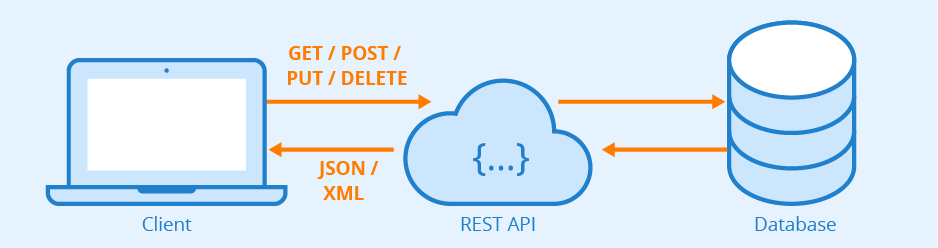
\includegraphics[width=11.5cm]{Image/Technical/RESTful_API.png}
        \caption{RESTful API}
        \label{RESTfulAPI}
    \end{center}
\end{figure}

REST hoạt động chủ yếu dựa vào giao thức HTTP chính sau:
\begin{itemize}
    \item GET (SELECT): Trả về một Resource hoặc danh sách Resource.
    \item POST (CREATE): Tạo mới một Resource.
    \item PUT (UPDATE): Cập nhật thông tin cho Resource.
    \item DELETE (DELETE): Xoá một Resource.
    \item PATCH: ghi đè các thông tin được thay đổi của đối tượng.
\end{itemize}

Ưu điểm của việc sử dụng RESTful API:
\begin{itemize}
    \item Code đơn giản và ngắn gọn giúp cho ứng dụng rõ ràng hơn
    \item Dữ liệu được trả về với nhiều định dạng khác nhau như: xml, html, json….
    \item REST URL đại diện cho resource chứ không phải hành động
    \item REST chú trọng vào tài nguyên của hệ thống.
\end{itemize}

Tuy nhiên vẫn còn tồn tại một số nhược điểm:
\begin{itemize}
    \item RESTful API rất khó thiết kế vì REST là kiểu kiến trúc và không phải công nghệ. Nó không có tiêu chuẩn quản lý, do đó không có quy tắc thiết kế nhanh và bền vững.
    \item Có rất nhiều thiết kế RESTful API khác nhau, khó đồng nhất.
\end{itemize}

\subsubsection{Token-Based Authentication}
Token-Based Authentication (xác thực dựa trên token) là một giao thức cho phép người dùng xác minh danh tính của mình và nhận mã token xác thực duy nhất. Trong thời gian tồn tại của mã token, người dùng có thể truy cập trang web hoặc ứng dụng mà không cần phải nhập lại thông tin đăng nhập. Mã token xác thực hoạt động giống như một vé được đóng dấu. Người dùng vẫn có quyền truy cập miễn là mã token vẫn còn hợp lệ. Sau khi người dùng đăng xuất hoặc thoát khỏi một ứng dụng, mã token sẽ bị vô hiệu hóa.\par

Xác thực dựa trên mã token khác với các kỹ thuật xác thực dựa trên mật khẩu hoặc dựa trên máy chủ truyền thống. Token cung cấp lớp bảo mật thứ hai và quản trị viên có quyền kiểm soát chi tiết đối với từng hành động và giao dịch.\par

\begin{figure}[h!]
    \begin{center}
        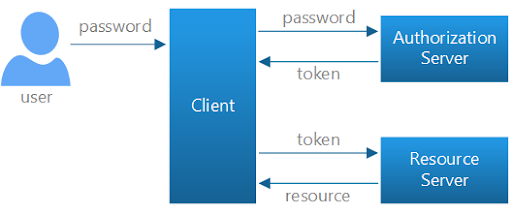
\includegraphics[width=12cm]{Image/Technical/token_auth.png}
        \caption{Token-Based Authentication}
        \label{TokenAuth}
    \end{center}
\end{figure}

Quá trình hoạt động:
\begin{itemize}
    \item Request: Người dùng yêu cầu quyền truy cập vào máy chủ hoặc tài nguyên được bảo vệ. Điều đó có thể liên quan đến đăng nhập bằng mật khẩu hoặc có thể liên quan đến một số quy trình khác.
    \item Verification: Máy chủ xác định rằng người đó phải có quyền truy cập. Điều đó có thể liên quan đến việc kiểm tra mật khẩu so với tên người dùng hoặc nó có thể liên quan đến một số quy trình khác.
    \item Tokens: Máy chủ giao tiếp với thiết bị xác thực. Sau khi xác minh, máy chủ phát hành một mã token và chuyển nó cho người dùng.
    \item Storage: Mã token nằm trong trình duyệt của người dùng trong khi công việc tiếp tục. Nếu người dùng cố gắng truy cập một phần khác của máy chủ, mã token sẽ giao tiếp lại với máy chủ để xác định quyền truy cập hoặc bị từ chối.
\end{itemize}
Quản trị viên đặt giới hạn cho mã token. Bạn có thể cho phép mã token dùng một lần bị hủy ngay lập tức khi người đó đăng xuất. Hoặc cũng có thể cho mã token tự hủy vào cuối một khoảng thời gian cụ thể.